\documentclass[simplex.tex]{subfiles}
% NO NEED TO INPUT PREAMBLES HERE
% packages are inherited; you can compile this on its own
\begin{document}
\subsection{Multiscale Network Testing for Two-Graph} 

We invented multiscale network test via diffusion maps and \texttt{MGC}, and extends its utility into testing two graphs of the same node set with different edge sets. Assume two graphs $\mathbf{G}_{1}$ and $\mathbf{G}_{2}$ are generated via a latent variable $\mathbf{u}_{i} = ( u_{1i}~ u_{2i}~ \cdots ~u_{5i} ) \in \mathbb{R}^{5}$ as follows:
\begin{equation}
\begin{split}
u_{ki} & \overset{i.i.d.}{\sim} Unif(0, 1), \quad i = 1,2, \ldots, n;~k = 1,2,\ldots, 5 \\
w_{i} & := (1- u_{i1} )^{2}, \quad i = 1,2, \ldots, n \\
A^{(1)}_{ij} \big| \mathbf{u}_{i}, \mathbf{u}_{j} & \sim Bernoulli \big( <\mathbf{u}_{i}/5, \mathbf{u}_{j}/5  > \big), \quad \forall i < j;~i,j=1,2,\ldots,n;~\mathbf{u}_{i}, \mathbf{u}_{j} \in \mathbb{R}^{5} \\
A^{(2)}_{ij} \big| w_{i}, w_{j} & \sim Bernoulli \big( <w_{i}, w_{j}  > \big), \quad \forall i < j;~i,j=1,2,\ldots,n.
\end{split}
\label{eq:twoGraphs}
\end{equation}
That is, Each graph is generated by a random dot product graph (RDPG), and the underlying dependency is reflected via the quadratic function of one-dimensional latent variable; this implies both multi-dimensional and nonlinear relationship where \texttt{MGC} is preferred to other benchmarks in testing network dependency in nodal attributes.  

\begin{figure}[h!]
\begin{cframed}
\centering
	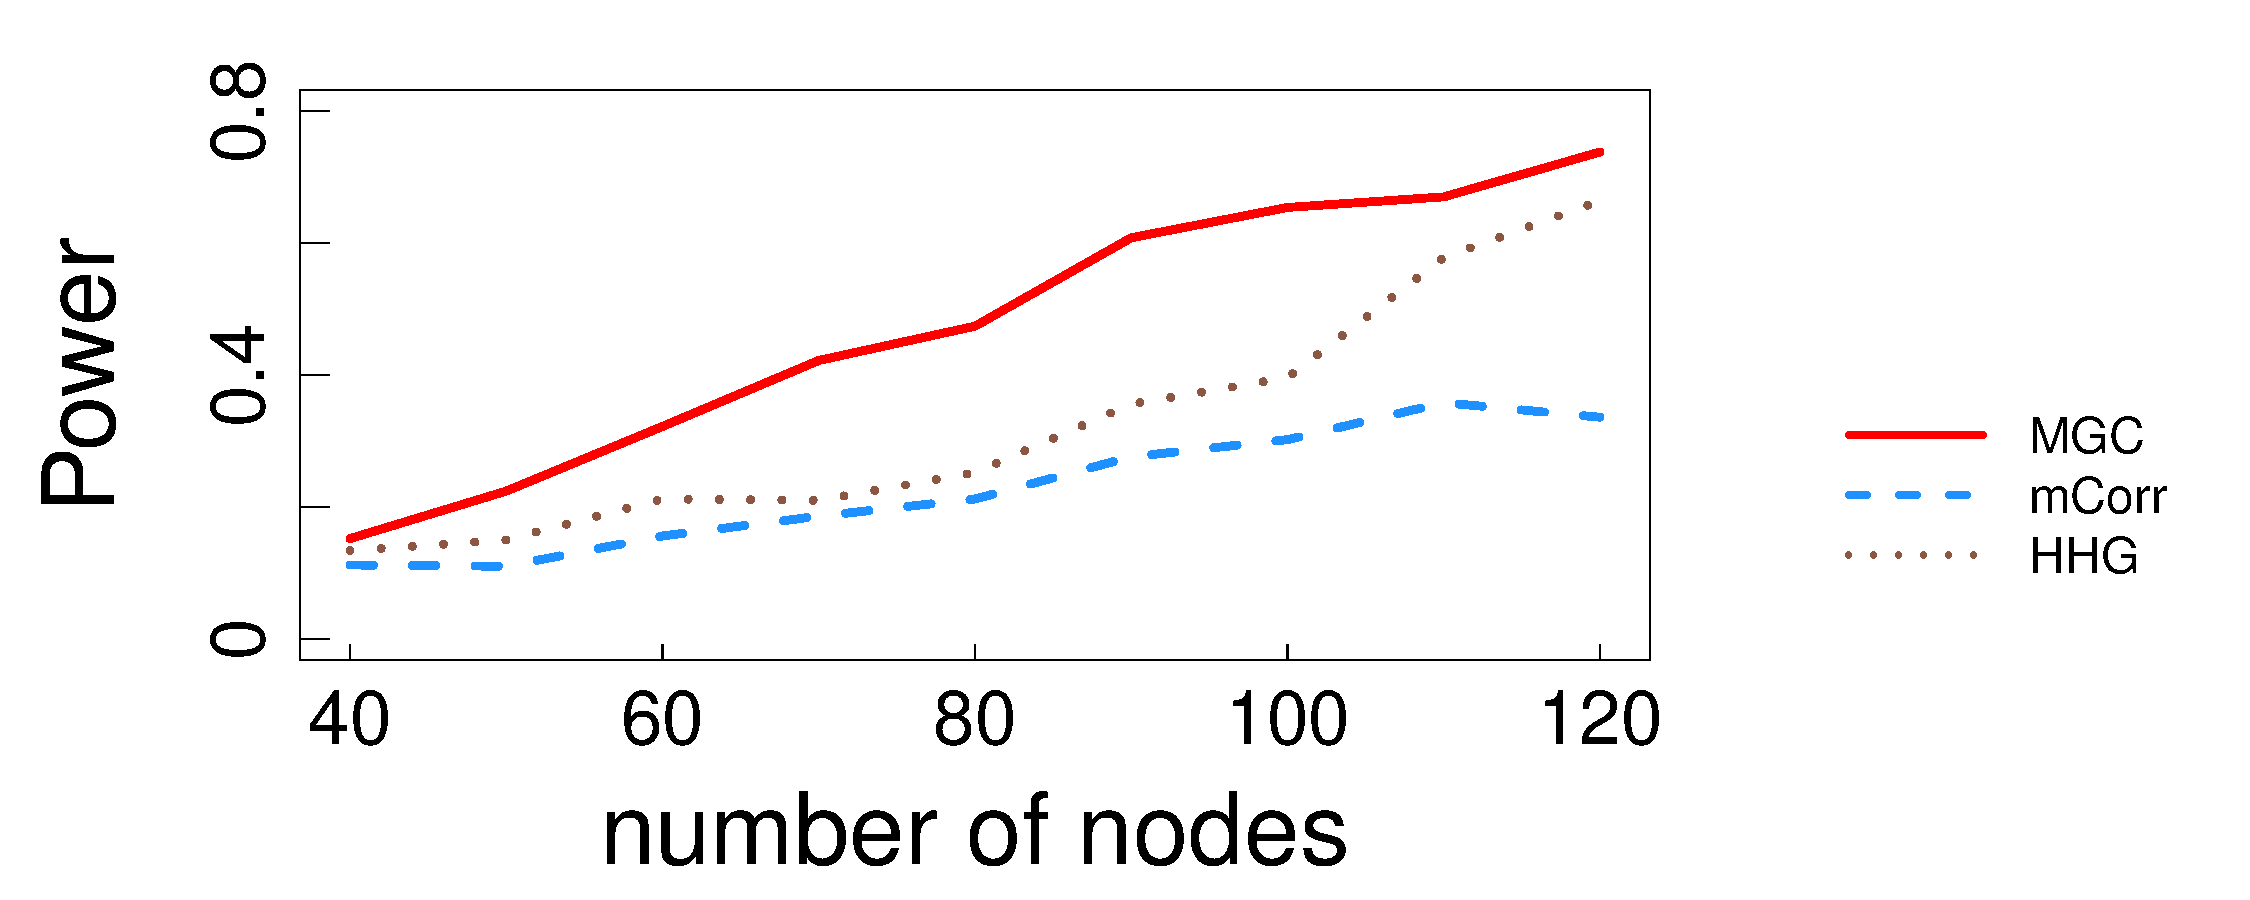
\includegraphics[width=0.7\textwidth]{../../figs/Graphs}
	\caption{The power curve with respect to increasing number of nodes for the two-graph dependency testing simulation (Equation~\ref{eq:twoGraphs}). The proposed approach achieves higher power than other methods.}
    \label{fig:graphtest}
		\end{cframed}
\end{figure}

Figure~\ref{fig:graphtest} shows the testing power of \texttt{MGC}, \texttt{mCorr}, and \texttt{HHG} against the number of nodes $n$, all based on the diffusion maps, and it demonstrates that the proposed approach is able to achieve higher testing power under relatively small number of nodes. Note that if noise is included in the set-up, or the nonlinear relationship is more complex than quadratic, the proposed approach still enjoys the same advantage, i.e., the testing power converges to $1$ faster than all other methods, though the actual number of nodes to achieve perfect power will likely increase under noisy and complex dependency.

The draft is submitted this month and available on arXiv.


\clearpage
\end{document}
